\documentclass[a4paper,12pt]{scrartcl}

\newcommand{\dropsign}[1]{\smash{\llap{\raisebox{-.5\normalbaselineskip}{$#1$\hspace{2\arraycolsep}}}}}%

\usepackage[utf8]{inputenc}
\usepackage[ngerman]{babel}
\usepackage{multicol}
\usepackage{scrpage2}\pagestyle{scrheadings}
\usepackage{graphicx} 
\usepackage{pgfplots}

\ihead{Blatt 4, G2B}
\chead{Elena Noll, Sven-Hendrik Haase, E. Böhmecke}
\ohead{\today}
\pagestyle{scrheadings}
\setheadsepline{1pt}
\setcounter{secnumdepth}{0}

\begin{document}

\section{Aufgabe 14}
\section{Aufgabe 15}
\section{Aufgabe 16}
\subsection{a)}
Das "Bit stuffing" wird im HDLC-Protokoll eingesetzt um zu vermeiden das innerhab des Datenbereichs bz der Prüfsumme das Opening bzw Closing flag (Bitfolge: 01111110) auftritt.
\begin{itemize}
	\item Bitfolge: 0011111110001111101
	\item Bitfolge nach dem "Bit stuffing": 001111101100011111001
\end{itemize}
\subsection{b)}
\subsection{c)}
Man kann mit Opening bzw. Closing Frames arbeiten. Somit weiß man wann ein Datenblock anfängt und wo er aufhört. Beim nächsten Opening Frame kann dann der jeweilige Block wieder Synchronisiert werden.
\subsection{d)}
\subsection{Ethernet}
Blocksynchronisation durch MAC-Frames (Media Access Control). Diese bestehen jeweils aus einer Präambel (7 Byte lange alternierende Bitfolge "101010...1010") gefolgt von einem Start Frame Delimeter (SFD). Die alternierende Bitfolge ermöglicht die Bitsynchronisation und das SFD (Blockanfang) der Blocksynchronisation.
\subsection{IEEE 802.11g WLANs}

\section{Aufgabe 17}
\subsection{a)}
\begin{itemize}
	\item Studen: ld(n)
	\item Knoten pro Stufe: n/2
\end{itemize}
\subsection{b)}
\begin{center}
  \makebox[\textwidth]{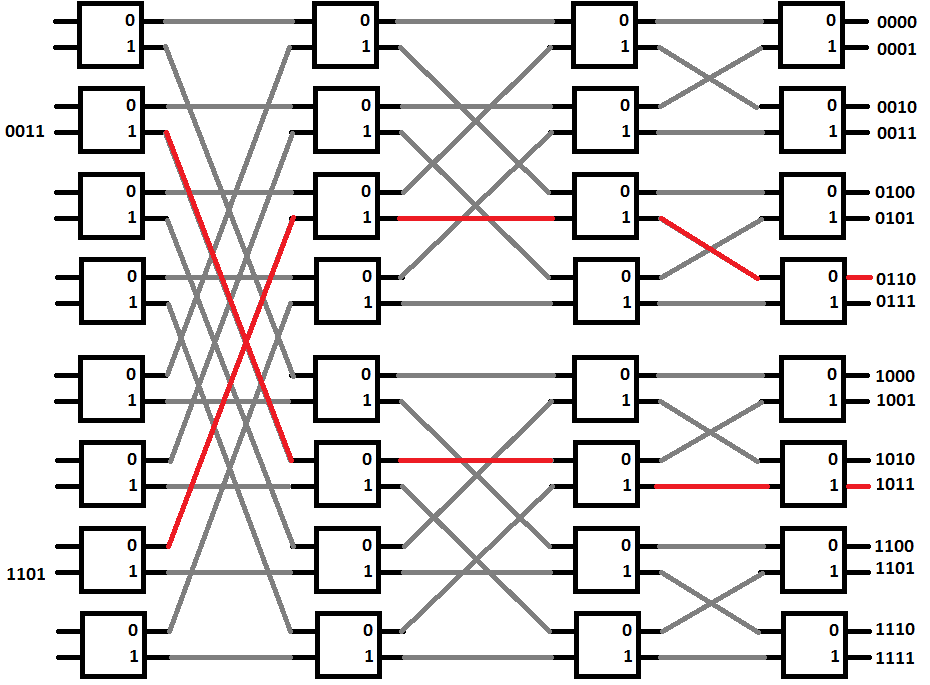
\includegraphics[width=\paperwidth]{./images/Blatt-4-Aufgabe17b}}
\end{center}
Die Zellen blockieren sich nicht auf dem Weg.
\subsection{c)}
Internet Blockierungen in einen Banyan-Netz lassen sich durch folgende Maßnahmen entschärfen:
\begin{itemize}
	\item Sort/Banyan-Netze: vorsortierung von Packeten sodass interne Blockierung vermieden wird
	\item Warteschlangen: Führt dazu dass die Leitung nur von jeweils eine Anfrage zur Zeit durchlässt.
\end{itemize}
\subsection{d)}
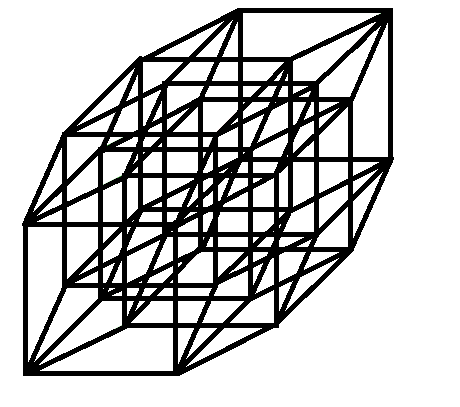
\includegraphics{./images/Blatt-4-Aufgabe17d}\\
Der 5-dimensionale Hperwürfel enthält 32 Knoten, 80 Verbindungen und 5 maximale "Hops" zwischen zwei Knoten. Da jeder Knoten 5 ausgehende Verbindungen jeweils hat, kann ein Ausfall von 5 Verbindung im ungünstigsten Fall bedeuten das 1 Knoten überhaupt nicht mehr durch eine Verbindung erreichtbar ist und somit ist auch nicht mehr sichergestellt das jeder mit jedem Knoten kommunizieren kann.
\subsection{e)}




\section{Aufgabe 10}
\subsection{a)}
Unter \textbf{Signalfunktion} versteht man z.B. die
Periodendauer des Signals.\\
Bei der \textbf{Spektralfunktion} betrachten wir
die Frequenzbänder zu einer bestimmten Zeit. Das
können wir mit dem Betrachten der Energie zu dieser
Zeit gleichsetzen.

\subsection{b)}
Es ist irrelevant, ob ein Signal mit Signalfunktion oder Spektralfunktion
dargestellt wird, die Signale sind mathematisch gleichwertig.\\

Wenn wir uns allerdins über das jeweils sinnvollere Anwendungsfeld unterhalten,
so ist zu bemerken, dass wir die Spektralfunktion immer dann benötigen,
wenn wir wissen möchten, wie hoch die Amplitude bestimmer Frequenzen des
Signals ist. Das ist z.B. bei vielen Audio- und Videoanwendungen relevant.
Dabei wird die Amplitude des bestimmer Frequenzbänder des Signals häufig
grafisch dargstellt. Das wäre mit der Signalfunktion nicht möglich.\\

Für die Sprachübertragung eignet sich die Signalfunktion eher, da wir hier
nicht an der diskreten Amplitude bestimmer Frequenzen interessiert sind,
sondern eher am Signal als Ganzem.

\subsection{c)}
Z in ASCII hat den Wert 90. In Binär 01011010.

\[ a_k=\frac{1}{\pi k} \left[\cos \frac{\pi k}{4} - \cos \frac{2 \pi k}{4} +
		\cos \frac{3 \pi k}{4} - \cos \frac{5 \pi k}{4} +
        \cos \frac{6 \pi k}{4} - \cos \frac{7 \pi k}{4} \right] \]

\[ b_k=\frac{1}{\pi k} \left[\sin \frac{2 \pi k}{4} - \sin \frac{\pi k}{4} +
		\sin \frac{5 \pi k}{4} - \cos \frac{3 \pi k}{4} +
        \sin \frac{7 \pi k}{4} - \sin \frac{6 \pi k}{4} \right] \]

\[ c=\frac{2}{T}*\frac{4}{8}T=\frac{1}{2} \]

\subsection{d)}
\begin{tabular}{l|l|l|l}
	k & \(a_k\) & \(b_k\) & \(h_k\) \\
    \hline
    1 & 3.533949646070574e-17 & -0.26369654378952473 & 0.26369654378952473 \\
    2 & -2.013073408267528e-17 & -5.847257748779064e-17 & 6.184083418561771e-17 \\
    3 & 1.884773144570973e-16 & -0.5123120295082292 & 0.5123120295082292 \\
    4 & 0.0 & 1.1694515497558127e-16 & 1.1694515497558127e-16 \\
    5 & -3.4632706531491627e-16 & 0.3073872177049376 & 0.3073872177049376 \\
    6 & 1.7915846815585113e-16 & -3.4912913180653474e-17 & 1.8252854083323783e-16 \\
    7 & -1.9689148028107485e-16 & 0.0376709348270749 & 0.0376709348270749 \\
    8 & 0.0 & -3.898171832519377e-17 & 3.898171832519377e-17
\end{tabular}
\\
\centerline{
\begin{tikzpicture}
	\begin{axis}[xlabel=\(k\),ylabel=\(h_k\),width=500pt,axis x line=middle, axis y line=center, tick align=outside]
		\addplot[mark=*,smooth] coordinates {
        	(1, 0.26369654378952473)
            (2, 6.184083418561771e-17)
            (3, 0.5123120295082292)
            (4, 1.1694515497558127e-16)
            (5, 0.3073872177049376)
            (6, 1.8252854083323783e-16)
            (7, 0.0376709348270749)
            (8, 3.898171832519377e-17)
        };
	\end{axis}
\end{tikzpicture}}

\section{Aufgabe 11}
\subsection{a)}
Der Begriff "Konstante Bitrate" (CBR) bezieht sich nicht auf das tatsächliche
Datenaufkommen, dass mit einem CBR-Codec encodiert wird, sondern auf die
beobachteten Daten, dort wo die Daten fließen (z.B. ein Internet-Stream).
Das heißt, dass die Daten, die aus dem CBR-Codec kommen, häufig gepaddet
werden müssen, um die CBR-Anforderungen zu erfüllen. Im Umkehrschluss heißt
das, dass die encodierten Daten in jedem Zeitsegment immer kleiner sein 
müsssen, als die gewünschte Bitrate, denn wir können immer neutrale Daten zum
padden benutzen, aber nichts wegnehmen, ohne dass es auffällt.

\subsection{b)}
\[FH_{Bit}(T) = \frac{1000}{1800000000000} = \frac{1}{1800000000}\]
mit T = 1 Std.

\subsection{c)}
Ja, kann man. Voraussetzung ist, dass die Bitfehlerhäufigkeit konstant bleibt.

\subsection{d)}
Da sich die Datenrate des Kanals verdoppelt aber die Bitfehlerhäufigkeit gleich beleiben soll, müssen sich die auftretenden Bitfehler auch verdoppeln. Da unsere Blockgröße L fest ist, wird die Wahrscheinlichkeit, dass in einem Block ein Fehler auftritt größer. Somit erhöht sich die Blockfehlerhäufigkeit.

\section{Aufgabe 12}
\subsection{a)}
\subsubsection{Definition 1}
Mit Jitter bezeichnet man in der Datenübertragung die Phasenschwankungen und damit die zeitlichen Änderungen von Signalfrequenzen. Es handelt sich um Schwankungen von fixierten Zeitpunkten z.B. dem Zeitpunkt des Übergangs von einer Signalamplitude eines Digitalsignals auf eine andere. Dadurch können sich Bezugszeitpunkte verschieben, was zu Fehlinterpretationen der Signale, zu Paketverlusten und damit zur Verschlechterung der Übertragungsqualität bei Echtzeitanwendungen führen kann. \\
\\
http://www.itwissen.info/definition/lexikon/Jitter-jitter.html

\subsubsection{Definition 2}
Als Jitter bezeichnet man das zeitliche Taktzittern bei der Übertragung von Digitalsignalen, eine leichte Genauigkeitsschwankung im Übertragungstakt (engl. Clock). Jitter ist als Störsignal im Normalfall unerwünscht. Allgemeiner ist Jitter in der Übertragungstechnik ein abrupter und unerwünschter Wechsel der Signalcharakteristik. Dies kann sowohl Amplitude als auch Frequenz und Phasenlage betreffen. Der Jitter ist die erste Ableitung einer Verzögerung (engl. Delay). Die spektrale Darstellung der zeitlichen Abweichungen wird als Phasenrauschen bezeichnet. Jitter ist nicht zu verwechseln mit Quantisierungsfehlern.
In der Netzwerktechnik wird mit Jitter außerdem die Varianz der Laufzeit von Datenpaketen bezeichnet. Dieser Effekt ist insbesondere bei Multimedia-Anwendungen im Internet (wie Internet-Radio und Internet-Telefonie) störend, da dadurch Pakete zu spät oder zu früh eintreffen können, um noch rechtzeitig mit ausgegeben werden zu können. Der Effekt wird durch einen sogenannten Jitterbuffer, einen speziellen „Datenpuffer“ reduziert, allerdings zum Preis von zusätzlicher Laufzeit, was vor allem bei Dialoganwendungen stört. Dieser Effekt spielt außerdem in der Prozessleittechnik eine Rolle. Kritische Prozessinformationen müssen innerhalb einer bestimmten Zeit verschickt und empfangen werden. Wird der Jitter zu groß, ist ein rechtzeitiges Eintreffen der kritischen Prozessinformationen nicht gewährleistet. \\
\\
http://de.wikipedia.org/wiki/Jitter

\subsubsection{Definition 3}
1) In voice over IP (VoIP), jitter is the variation in the time between packets arriving, caused by network congestion, timing drift, or route changes. A jitter buffer can be used to handle jitter. \\
\\
2) Jitter is the deviation in or displacement of some aspect of the pulses in a high-frequency digital signal. As the name suggests, jitter can be thought of as shaky pulses. The deviation can be in terms of amplitude, phase timing, or the width of the signal pulse. Another definition is that it is "the period frequency displacement of the signal from its ideal location." Among the causes of jitter are electromagnetic interference (EMI) and crosstalk with other signals. Jitter can cause a display monitor to flicker; affect the ability of the processor in a personal computer to perform as intended; introduce clicks or other undesired effects in audio signals, and loss of transmitted data between network devices. The amount of allowable jitter depends greatly on the application.\\
\\
http://searchunifiedcommunications.techtarget.com/definition/jitter

\subsubsection{Berechnung des Jitter-Wertes}
Nach http://www.crn.de/netzwerke-tk/artikel-84415.html
\[Jitter = (19 - 12 - 16 - 16 - 13 - 14 - 17 - 13 - 12 - 10) - (1 - 2 - 3 - 4 - 5 - 6 - 7 - 8 - 9 - 10) = -51\]

\subsection{b)}
Es ist für den interaktiven Multimediaeinsatz schlechthin konstituierend, dass
zumindest die Latenz einigermaßen abschätzbar bleibt. Software wie Skype
beispielsweise wechselt bei zu hohen Latenzen oder zu viel Paketverlust
automatisch auf eine schlechtere Qualitätsstufe, damit die Grundfunktion erhalten
bleibt.

\newpage
\section{Aufgabe 13}
\subsection{a)}
\begin{verbatim}
Zu übertragene GOP:           I B B P B B P B B
Fehlerhafte Frames:           B       P
Korrekt decodierbare Frames:  I   B P B B
\end{verbatim}

\subsection{c)}
Ein Paketverlust kommt in der realen Welt selten allein. Bei Hardwareschäden
fallen beliebig viele Pakete direkt nacheinander weg. Ebenfalls bei
Überlastung von Datenverbindungen, wobei viele Pakete erst viel zu spät ankommen
oder gar fallen gelassen werden, weil der Buffer im betroffenen Gateway
überläuft. Auch kann es sein, dass das physische Übertragungsmedium gestört
wird. Das kann beispielsweise durch Radiowellen- oder Magnetinterferenzen
ausgelöst werden.

\end{document}
